\documentclass{beamer}

\usetheme{Madrid} 
\usepackage{graphicx} % Required for including images
\usepackage{url}
\usepackage{setspace} % Ensure setspace is loaded (recommended)
\usepackage{tikz} % <<< Add tikz package

% --- Customize Footline ---
\setbeamertemplate{footline}{%
  \leavevmode
  \hbox{
    \begin{beamercolorbox}[wd=0.25\paperwidth, ht=2.25ex, dp=1ex, center]{author in head/foot}%
      \usebeamerfont{author in head/foot}\insertshortauthor, \insertshortinstitute
    \end{beamercolorbox}%
    \begin{beamercolorbox}[wd=0.5\paperwidth, ht=2.25ex, dp=1ex, center]{title in head/foot}%
      \usebeamerfont{title in head/foot}\insertshorttitle
    \end{beamercolorbox}%
    \begin{beamercolorbox}[wd=0.25\paperwidth, ht=2.25ex, dp=1ex, right]{date in head/foot}%
      \usebeamerfont{date in head/foot}\insertshortdate{}\hspace*{2em} \insertframenumber{} / \inserttotalframenumber \hspace{2ex}
    \end{beamercolorbox}%
  }%
  \vskip0pt
}
% --- End Footline Customization ---

\setbeamerfont{caption}{size=\tiny}
\setlength\abovecaptionskip{1pt}

\title{A review of \textbf{Segment Anything (SAM)}, 2023}
\author{Zachary Parent}
\date{6th of May, 2025}
\institute{UPC - UB}


\begin{document}

\begin{frame}
    \titlepage

    \begin{tikzpicture}[remember picture, overlay]
        \node[anchor=west, 
              inner sep=0pt, 
              yshift=-1.6cm]   
             at ([xshift=16pt]current page.west) 
             {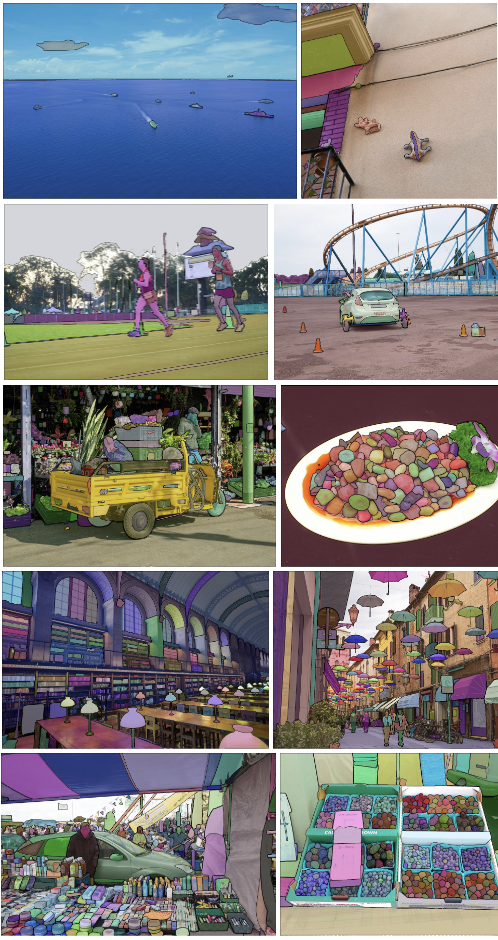
\includegraphics[height=0.55\textheight]{figures/examples_left.png}}; 

        \node[anchor=east, 
              inner sep=0pt, 
              yshift=-1.6cm]   
             at ([xshift=-16pt]current page.east) 
             {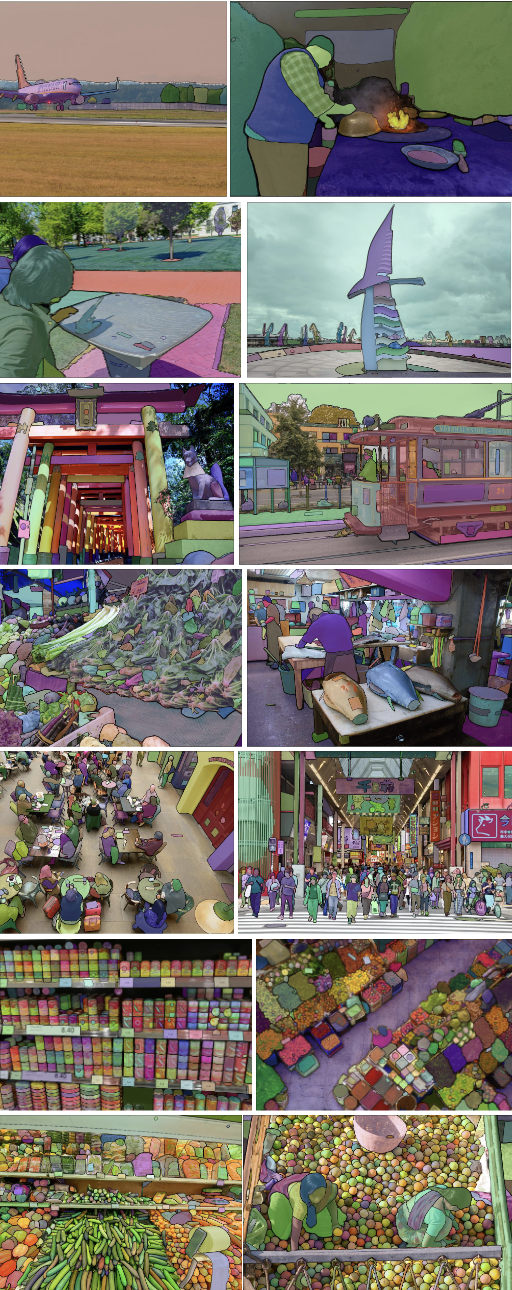
\includegraphics[height=0.55\textheight]{figures/examples_right.png}}; 
    \end{tikzpicture}
\end{frame}

\begin{frame}{Outline}
    \tableofcontents
\end{frame}

\section{Introduction}

\begin{frame}{The Vision: A Foundation Model for Segmentation}
    \frametitle{The Vision: A Foundation Model for Segmentation}
    Goal: Build a foundation model analogous to LLMs for vision, specifically for segmentation.
    \begin{itemize}
        \item Like GPT, but for pixels.
        \item Enables zero-shot generalization via prompt engineering.
        \item Three core components: Task, Model, Dataset.
    \end{itemize}
    Released model (SAM) and dataset (SA-1B) to foster research.
\end{frame}

\begin{frame}{Key Research Questions}
    \frametitle{Key Research Questions}
    \begin{enumerate}
        \item What task will enable zero-shot generalization?
        \item What is the corresponding model architecture?
        \item What data can power this task and model?
    \end{enumerate}
    \begin{figure}
        \centering
        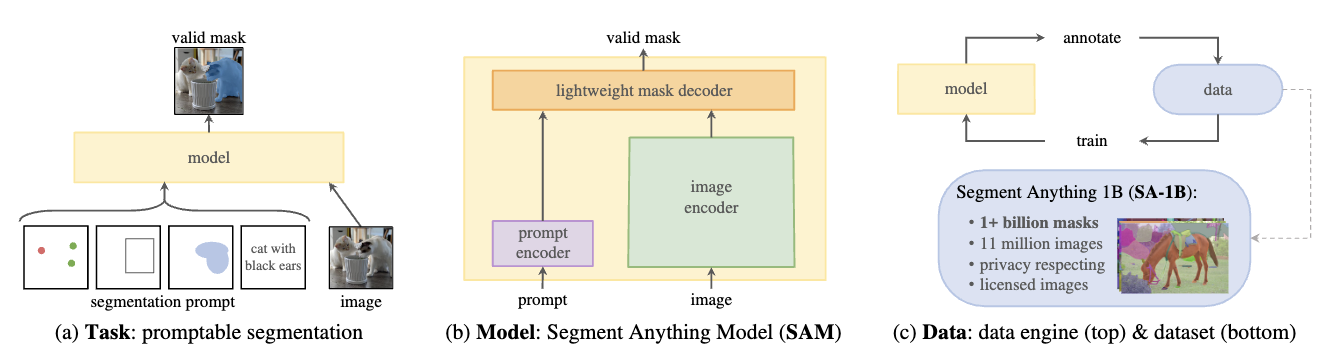
\includegraphics[width=0.8\textwidth]{figures/SA_overview.png}
        \caption{We aim to build a foundation model for segmentation by introducing three interconnected components: a prompt-
        able segmentation task, a segmentation model (SAM) that powers data annotation and enables zero-shot transfer to a range
        of tasks via prompt engineering, and a data engine for collecting SA-1B, our dataset of over 1 billion masks.}
    \end{figure}
    %% TODO: fix the caption sizing
\end{frame}

\section{The Task: Promptable Segmentation}

\begin{frame}{Defining the Task}
    \frametitle{Defining the Task: Promptable Segmentation}
    \textbf{Input:} An image and a prompt (point, box, mask, text). \\
    \textbf{Output:} A valid segmentation mask.
    \begin{itemize}
        \item "Valid" means outputting a reasonable mask even if the prompt is ambiguous.
        \item Inspired by interactive segmentation, but goal is always predicting a valid mask immediately.
    \end{itemize}
    \vfill
    
    \begin{figure}
        \centering
        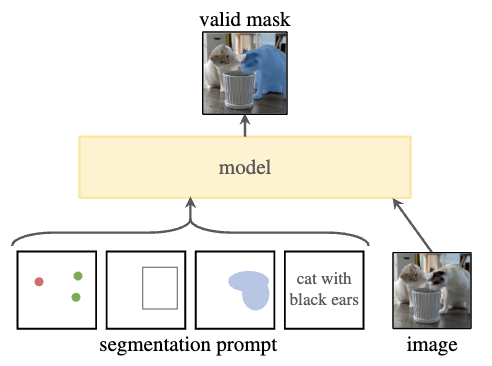
\includegraphics[width=0.4\textwidth]{figures/prompt_types.png}
        \caption{Prompt types (a) Point prompts (b) Box prompts (c) Mask prompts (d) Text prompts.}
    \end{figure}
    %% TODO: fix the caption sizing
\end{frame}

\begin{frame}{Zero-Shot Transfer via Prompting}
    \frametitle{Zero-Shot Transfer via Prompting}
    The core idea: Train a model on the general promptable task, then solve specific downstream tasks by designing the right prompts.
    \begin{itemize}
        \item Example: Use bounding box outputs from a cat detector as prompts to get cat instance segmentation.
        \item SAM acts as a composable component in a larger system.
        \item Can adapt to many (but not all) existing and new tasks.
    \end{itemize}
\end{frame}

\section{The Model: SAM Architecture}

\begin{frame}{Model Requirements & Design}
    \frametitle{Model Requirements \& Design}
    \textbf{Requirements:}
    \begin{itemize}
        \item Flexible Prompts: Handle various input types.
        \item Real-time: Amortized real-time inference ($\sim$50ms) for interactivity.
        \item Ambiguity-aware: Output multiple masks for ambiguous prompts.
    \end{itemize}
    \textbf{Design:} Decoupled architecture for efficiency.
    \begin{enumerate}
        \item Heavyweight Image Encoder (ViT-H MAE pre-trained) - 1x per image.
        \item Lightweight Prompt Encoder (Positional embeddings, CLIP for text).
        \item Lightweight Mask Decoder (Transformer) - combines image and prompt embeddings.
    \end{enumerate}
    \vfill
    \begin{figure}
        \centering
        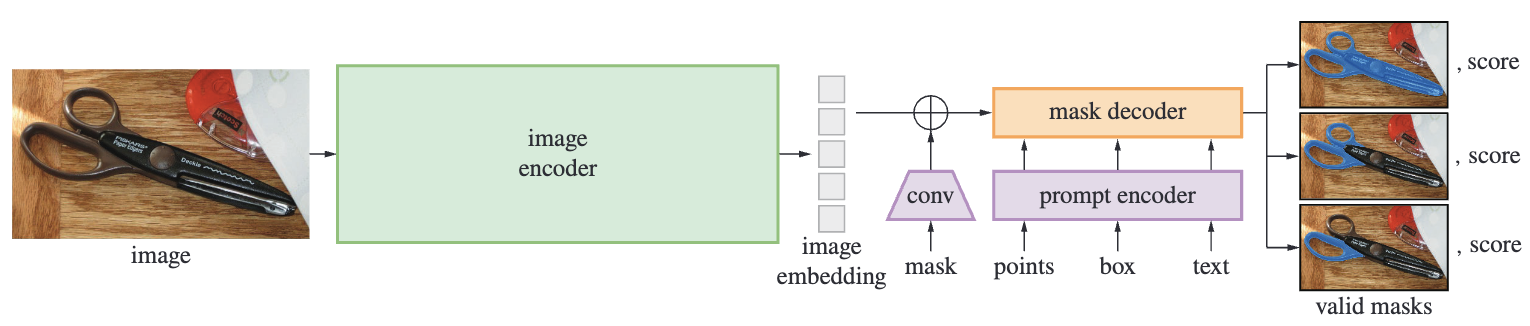
\includegraphics[width=0.8\textwidth]{figures/SAM_overview.png}
        \caption{Segment Anything Model (SAM) overview. A heavyweight image encoder outputs an image embedding that can
        then be efficiently queried by a variety of input prompts to produce object masks at amortized real-time speed. For ambiguous
        prompts corresponding to more than one object, SAM can output multiple valid masks and associated confidence scores.}
        \label{fig:sam_architecture}
    \end{figure}
    %% TODO: fix the caption sizing
\end{frame}

\begin{frame}{Encoder/Decoder Details}
    \frametitle{Encoder/Decoder Details}
    \textbf{Image Encoder:} MAE pre-trained ViT.
    \textbf{Prompt Encoder:}
    \begin{itemize}
        \item Sparse (Points, Boxes, Text): Positional encodings + learned embeddings per prompt type. Text uses CLIP.
        \item Dense (Masks): CNN downscales mask, combines with image embedding.
    \end{itemize}
    \textbf{Mask Decoder:}
    \begin{itemize}
        \item Transformer decoder updates prompt tokens via self/cross-attention.
        \item Upscales image embedding.
        \item Predicts mask logits via MLP + dynamic linear classifier using output tokens.
    \end{itemize}
    Loss: Linear combination of Focal Loss and Dice Loss.
\end{frame}


\section{The Dataset: SA-1B}

\begin{frame}{The Need for Data \& The Data Engine}
    \frametitle{The Need for Data \& The Data Engine}
    Problem: No web-scale segmentation data exists.
    Solution: Build a "Data Engine" - iterate between model-assisted annotation and model improvement.
    \textbf{Three Stages:}
    \begin{enumerate}
        \item \textbf{Assisted-Manual:} Annotators label interactively with SAM's help. Model retrained iteratively.
        \item \textbf{Semi-Automatic:} SAM proposes masks for likely objects; annotators focus on the rest.
        \item \textbf{Fully Automatic:} Prompt SAM with a regular grid (32x32) of points $\rightarrow$ ~100 masks/image.
    \end{enumerate}
    \vfill
    \begin{figure}
        \centering
        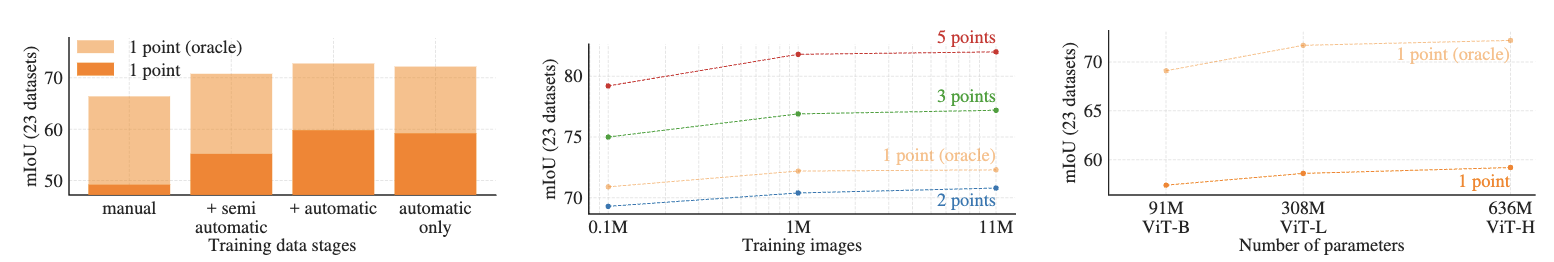
\includegraphics[width=0.8\textwidth]{figures/data_engine_ablation.png}
        \caption{Ablation studies of our data engine stages, image encoder scaling, and training data scaling. (Left) Each data
        engine stage leads to improvements on our 23 dataset suite, and training with only the automatic data (our default) yields
        similar results to using data from all three stages. (Middle) SAM trained with $\sim$10\% of SA-1B and full SA-1B is comparable.
        We train with all 11M images by default, but using 1M images is a reasonable practical setting. (Right) Scaling SAM's image
        encoder shows meaningful, yet saturating gains. Nevertheless, smaller image encoders may be preferred in certain settings.}
        \label{fig:data_engine}
    \end{figure}
    %% TODO: fix the caption sizing
\end{frame}

\begin{frame}{SA-1B Dataset}
    \frametitle{SA-1B Dataset}
    Result of the fully automatic stage.
    \begin{itemize}
        \item \textbf{1.1 Billion} high-quality masks.
        \item \textbf{11 Million} diverse, high-resolution images (licensed from provider).
        \item \textbf{400x} more masks than previous largest datasets (COCO, LVIS).
        \item Masks automatically generated and filtered for quality/stability (IoU, stability threshold).
        \item Geographically and economically diverse image sources.
    \end{itemize}
    \begin{figure}
        \centering
        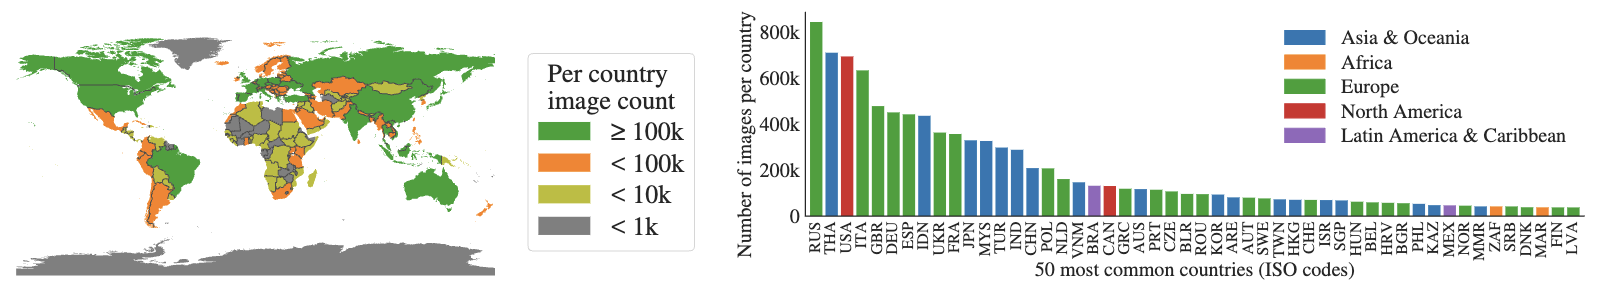
\includegraphics[width=0.8\textwidth]{figures/source_geography.png}
        \caption{Estimated geographic distribution of SA-1B images. Most of the world's countries have more than 1000 images in
        SA-1B, and the three countries with the most images are from different parts of the world.}
        \label{fig:source_geography}
    \end{figure}
    %% TODO: fix the caption sizing
\end{frame}

\section{Evaluation \& Results}

\begin{frame}{Zero-Shot Evaluation}
    \frametitle{Zero-Shot Evaluation}
    Extensive evaluation on 23 diverse segmentation datasets.
    \begin{itemize}
        \item Single point prompt performance often near manually annotated GT.
        \item Strong results on zero-shot downstream tasks via prompt engineering:
        \vspace{-1em}
        \begin{itemize}
            \item Edge Detection
            \item Object Proposal Generation
            \item Instance Segmentation
            \item Text-to-Mask (preliminary)
        \end{itemize}
    \end{itemize}
    \begin{figure}
        \centering
        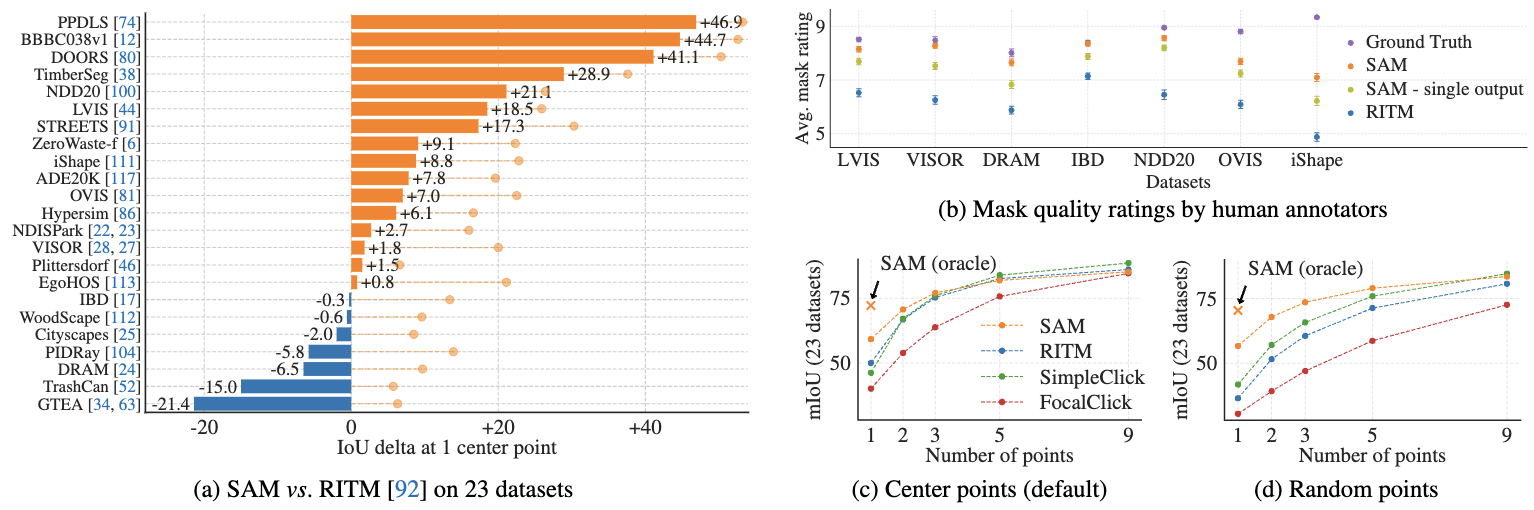
\includegraphics[width=0.8\textwidth]{figures/zero_shot_performance.png}
        \caption{Point to mask evaluation on 23 datasets. (a) Mean IoU of SAM and the strongest single point segmenter, RITM [92].
        Due to ambiguity, a single mask may not match ground truth; circles show "oracle" results of the most relevant of SAM's 3
        predictions. (b) Per-dataset comparison of mask quality ratings by annotators from 1 (worst) to 10 (best). All methods use
        the ground truth mask center as the prompt. (c, d) mIoU with varying number of points. SAM significantly outperforms prior
        interactive segmenters with 1 point and is on par with more points. Low absolute mIoU at 1 point is the result of ambiguity.}
        \label{fig:zero_shot_performance}
    \end{figure}
    %% TODO: fix the caption sizing
\end{frame}

\section{Strengths}

\begin{frame}{Strengths}
    \frametitle{Strengths}
    \begin{itemize}
        \item \textbf{Foundation Model Vision:} Pioneering promptable, general segmentation.
        \item \textbf{Unifying Task:} Promptable segmentation enables flexibility and zero-shot transfer.
        \item \textbf{Massive Dataset (SA-1B):} Unprecedented scale and diversity.
        \item \textbf{Strong Zero-Shot Performance:} Impressive generalization across many tasks/datasets.
        \item \textbf{Efficient Architecture:} Decoupled design allows real-time interaction.
    \end{itemize}
\end{frame}

\section{Limitations \& Future Work}

\begin{frame}{Limitations \& Future Work}
    \frametitle{Limitations \& Future Work}
    \begin{itemize}
        \item \textbf{Dataset Quality Assurance:} Transparency needed on automated mask filtering effectiveness.
        \item \textbf{Downstream Implementation:} Lack of practical integration examples.
        \item \textbf{Prompt Engineering:} Methodology underexplored.
        \item \textbf{Shallow Semantics:} Text understanding needs improvement.
        \item \textbf{Bias Analysis:} Surface-level; deeper sociotechnical audit needed.
        \item \textbf{Generalist vs Specialist:} May not beat specialized models in niche domains.
    \end{itemize}
\end{frame}

\section{Conclusion}

\begin{frame}{Conclusion}
    \frametitle{Conclusion}
    Segment Anything introduces a powerful new paradigm for image segmentation.
    \begin{itemize}
        \item Successfully implements a promptable task, model, and large-scale dataset.
        \item Demonstrates strong zero-shot capabilities.
        \item Opens up many avenues for future research in foundation models for vision, prompt engineering, and dataset quality.
    \end{itemize}
    A significant step towards general-purpose, interactive image understanding.
\end{frame}

\begin{frame}{Thank You / Q&A}
    \frametitle{Thank You / Q\&A}
    \centering
    {\Large\textbf{Questions?}}
    \vfill
    Model and dataset available at: \\ \url{https://segment-anything.com}
\end{frame}


\end{document}
